\chapter{The RPC Muon Detector}\label{chap:RPC}

%The development of Resistive Plate Chamber (RPC) was first motivated by the need to improve detectors' timing characteristic. The first improvement was Pestov spark counter developed by Yu.N. Pestov and G.V. Fedotovich. Later on the great simplification of the realization of the concepts of Pestov counter introduced in 1981 by R. Santonico and R. Cardarelli~\cite{Santonico1981} leads to RPC. RPCs are simple in structure and cheap to manufacture, operate and scale up. RPCs have played an important role in many particle physics experiments like BaBar and LHC. The Daya Bay project also adopts the RPC as a part of the muon system.
Resistive Plate Chambers (RPCs) are planar gas detectors which have good timing resolution~\cite{Santonico1981}. RPCs are simple in structure and cheap to manufacture, easy to operate and scale up. RPCs have played an important role in many particle physics experiments BaBar, LHC, and BESIII~\cite{Han2008}. The Daya Bay project adopts the BESIII RPC as the muon top tracker.


\section{RPC bare chambers}
A RPC, called bare chamber in Daya Bay, is a parallel plate gas detector for detecting charged particles. The structure of a Daya Bay RPC bare chamber is shown in Figure~\ref{fig:rpcstruct}. A Daya Bay RPC bare chamber is formed by two 2 mm bakelite sheets~\cite{Zhang2007} separated by spacers in a 10 cm $\times$ 10 cm grid to form a 2 mm gas gap. The spacer has a disk-shaped mid-section of 12 mm to decrease the surface current.
\begin{figure}
	\centering
	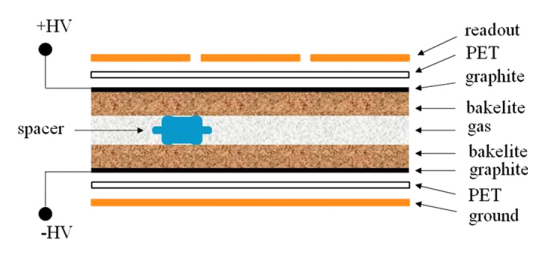
\includegraphics[width=.6\textwidth]{figures/chap5/RPC_Structure.eps}
	\caption{The structure of a Daya Bay RPC bare chamber.}
	\label{fig:rpcstruct}
\end{figure}
The total area of the button-shaped spacers occupy no more than $1\%$ of the area of a RPC bare chamber to minimize the dead area. Each bakelite sheet is coated with graphite~\cite{Ma2010} on the outside to serve as the electrode. A high voltage is applied between the two electrodes. The signal is read from readout strips from the outside. On top of the graphite there is a layer of Mylar film whose composition is polyethylene terephthalate (PET) to insulate the readout strips against the electrode and protect the graphite coating from scratching. The readout strips and ground plane are made from sheets of copper-clad FR-4. The signals are read out from the positive high voltage side.

\subsection{RPC Quality Control and Quality Assurance}
The bakelite sheets are made by Li Shen Wood Product Inc. factory in Xinji City~\cite{Ma2011}. The bakelite is made from paper soaked in phenolic and melaminic resins. The top layer is made with finer paper and melaminic coating. The error in the thickness of the sheets is within $1\%$. The length and width are about 230 cm and 120 cm. After production, the sheets were sent to IHEP, and the bulk resistivity of the sheets was measured. Four kV voltage was applied across 2 circular electrodes of 5 cm diameter, and the current was recorded to determine the resistivity. Since the measurement was done in a room without temperature control, the resistivity at 20\degree C is obtained by the following formula
\begin{equation}
	\rho_{20}=\rho_T\times 10^{0.06(T-20)}
\end{equation}
where $\rho_T$ is the resistivity measure at temperature $T$ in degrees Celsius, and 0.06 is an empirical parameter. Only bakelite sheets with resistivity in the range of 0.5-2.5 $\Omega$cm at 20 degrees Celsius are accepted and used in the module assembly. The bulk resistivity is related to the RPC performance. Higher resistivity leads to lower current and singles rate. However, when the RPC is hit by a charged particle, charges accumulate in the electrodes and then dissipate like the discharge of a capacitor. The charge in the dielectric electrodes, i.e. bakelite, follows an exponential decay $Q(t)=Q_0e^{-t/\tau}$ with a time constant $\tau=RC=\left(\rho\frac{d}{A}\right)\left(\epsilon\frac{A}{d}\right)=\rho\epsilon$, where $R$ is the resistance, $C$ is the capacitance, $d$ is the thickness, $A$ is the area, $\rho$ is the bulk resistivity, and $\epsilon$ is the permittivity of the bakelite. Therefore a larger resistivity means a longer charge relaxation time, leading to a lower detector efficiency because the area is dead. However, higher resistivity also leads to lower dark current. Since the counting rate at Daya Bay is relatively low, a higher resistivity is reasonable, but not so high as to reduce the efficiency significantly.

Bakelite sheets that passed the test were sent to Gaonengkedi Ltd. Co. (GNKD)~\cite{Ma2011} in Beijing for RPC chamber assembly. First, they were cut into 1$\times$2.1 m$^2$ and 1.1$\times$2.1 m$^2$ sheets for small and big RPCs, respectively. The size of the RPC is assured to be within $0.1\%$. A thin layer of graphite was coated on the surface of bakelite sheets, leaving 1 cm of space from the four edges. The graphite surface resistivity is required to be in the range of 400-1000 $k\Omega/\Box$. A piece of copper tape was attached to one of its corners for high voltage connection. Then a 100 $\mu m$-thick PET film covered the side of graphite coating for protection and insulation.

After the bakelite sheets were properly prepared, they were assembled into RPC chambers. First segmented edge spacers, made of the thermoplastic ABS, of size 10 mm wide and 2 mm thick, were glued along the perimeter of the bakelite sheet on the side without graphite coating. Two gas feedthroughs, also made of ABS, were embedded in the two short sides around the corners, diagonally across the sheet adjacent to the copper tape. After that the disk-shaped polycarbonate spacers were glued to the same side without graphite coating in a 10 cm $\times$ 10 cm grid, another bakelite sheet was glued on top of the spacers to form a chamber. In the first 2 hours after the chamber was sealed, the pressure in the chamber was lowered to about $8\%$ atmospheric pressure to ensure good glue cure. A $<0.1\%$ leak rate was required, and failed RPCs were glued again along the perimeter and tested again. Finally for each gas feedthrough a high voltage pin was soldered inside and made contact with the copper tape. The exposed copper tape and solder were then covered by insulating epoxy.

Newly made RPCs usually have a noise rate so high that it lowers the efficiency. It is known~\cite{ZhangJiawen2007} that a so-called training process can bring the noise down to a stable and acceptable rate. The training is done by applying the high voltage on RPC up to 10 kV for at least 48 hours, and flowing pure argon without other quenching gas so that the current can reach 2-3 orders of magnitude higher than that of normal operation condition. The training process burns off dust and ``polishes'' the surfaces. Figure~\ref{fig:training_current} shows the training current of a sample of 7 RPCs.
\begin{figure}[ht]
	\centering
	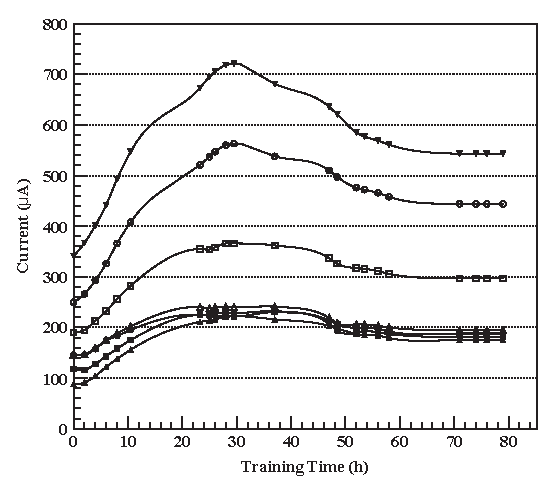
\includegraphics[width=.7\textwidth]{figures/chap5/training_current.eps}
	\caption{Training current of 7 RPCs.}
	\label{fig:training_current}
\end{figure}
We see that the current rises in the beginning and then drops off to a steady value. After training, when the RPC is put to use and operated in normal condition, the current is usually reduced by a factor of 10 compared with RPCs which are not trained.

%A gas combination of Ar, isobutane and R-134A flows in the gap. When charged particles pass through the gas gap, Ar molecules are ionized and the released electrons then undergo acceleration by the applied electric field. This primary electron then ionizes other Ar molecules and generates an electron avalanche. When the avalanche electrons drift the the anode, they induce electric signals which can then be readout. The isobutane can absorb ultraviolet photons and prevents a secondary streamer. The R-134A has high electron affinity and can restrict the size of the streamer.


\section{RPC Modules}
The RPC arrays in EH1 and EH2 are composed of 6 rows $\times$ 9 columns of RPC modules while that in EH3 is composed of 9 rows $\times$ 9 columns of RPC modules. Each module is an aluminum box of dimensions 2.17m $\times$ 2.20m $\times$ 0.08m containing bare chambers, insulating materials, support panels, readout strips, and ground planes. The RPC modules sit on the support structure which can be moved to an ``RPC hall'' next to the water pool during the AD and water pool installation. At each site, two additional RPC modules are installed at two opposing sides of the water pool, around two meters above the RPC array. Figure~\ref{fig:support_structure} shows the arrangement of the RPC modules on the support structure and the axes for defining the rows and columns of a RPC module.
\begin{figure}
	\centering
	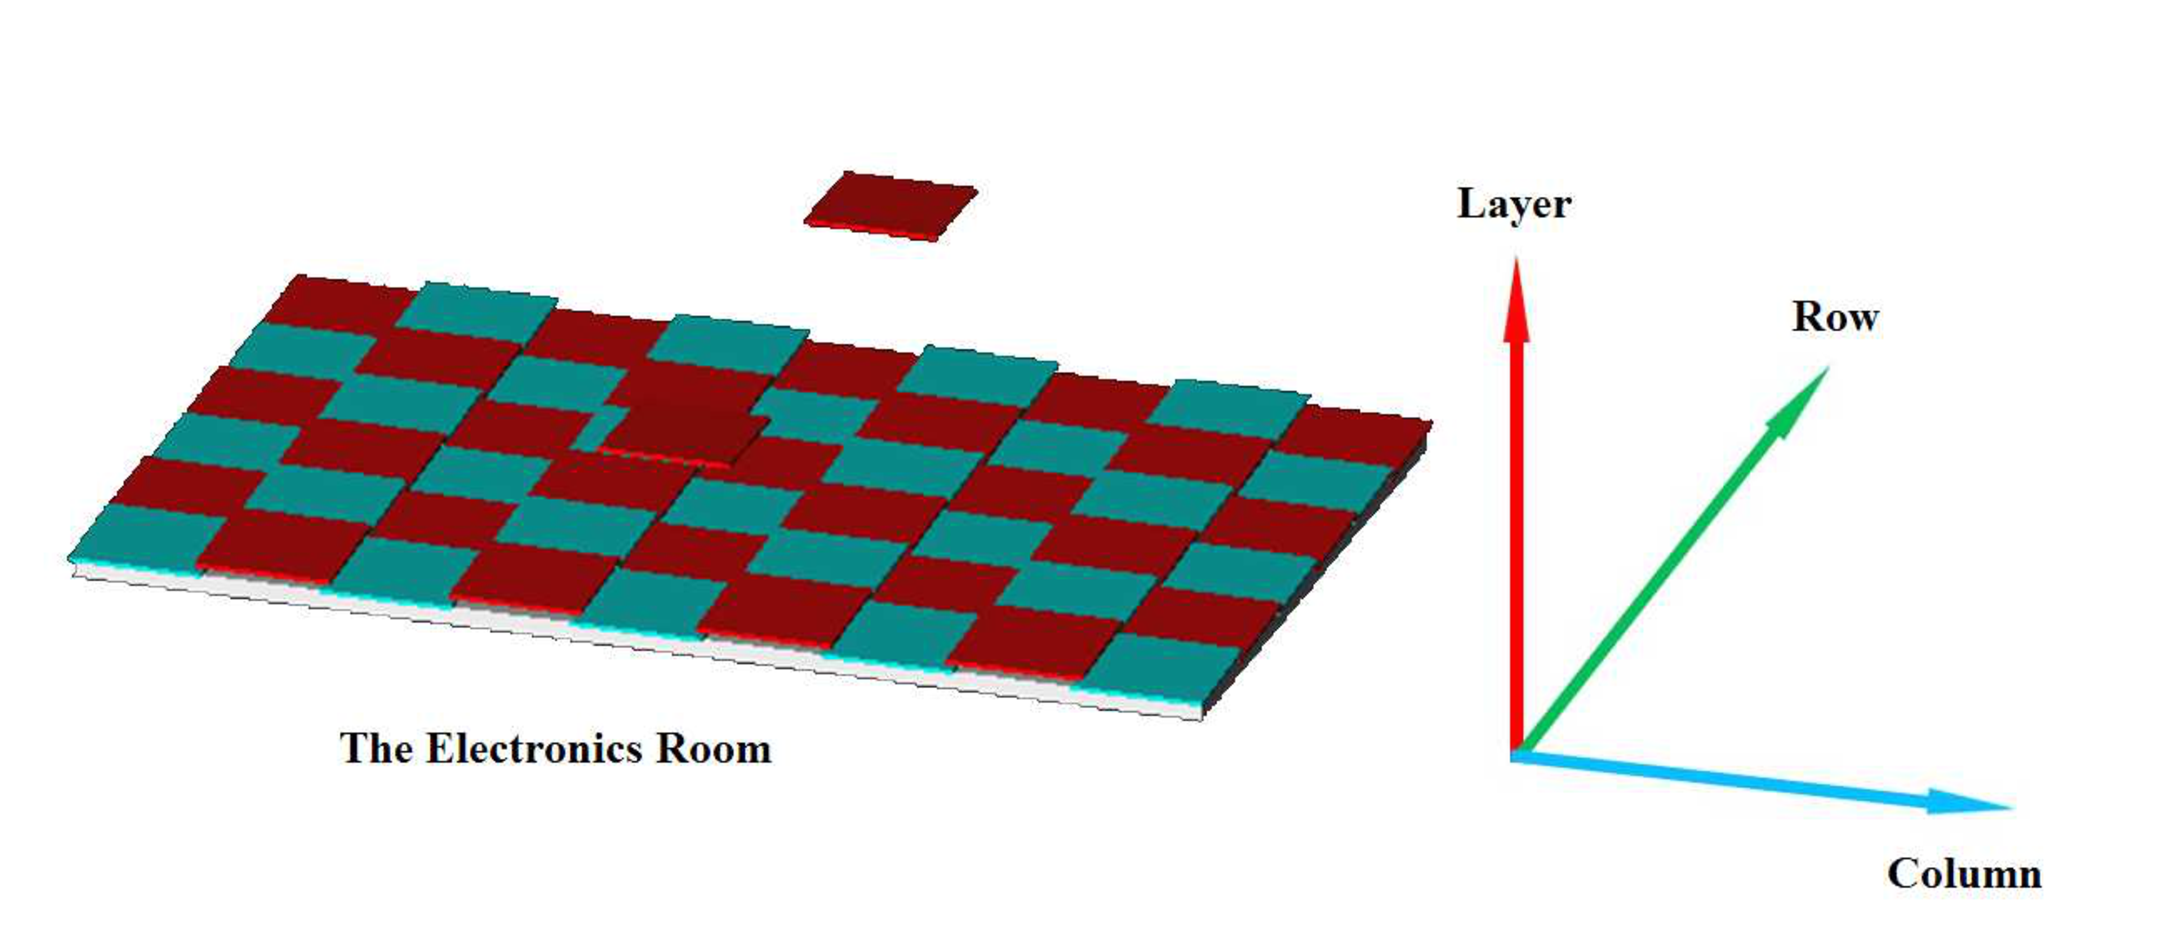
\includegraphics[width=0.7\textwidth]{figures/chap5/support_structure.eps}
	\caption{The arrangement of the RPC modules on the support structure and the convention used for locating a RPC module.}
	\label{fig:support_structure}
\end{figure}
Note that there is a 10 cm overlap on all sides of adjacent modules aiming at minimizing the dead regions. The inner structure of a Daya Bay RPC module is shown in Figure~\ref{fig:module_inner_structure}.
\begin{figure}
	\centering
	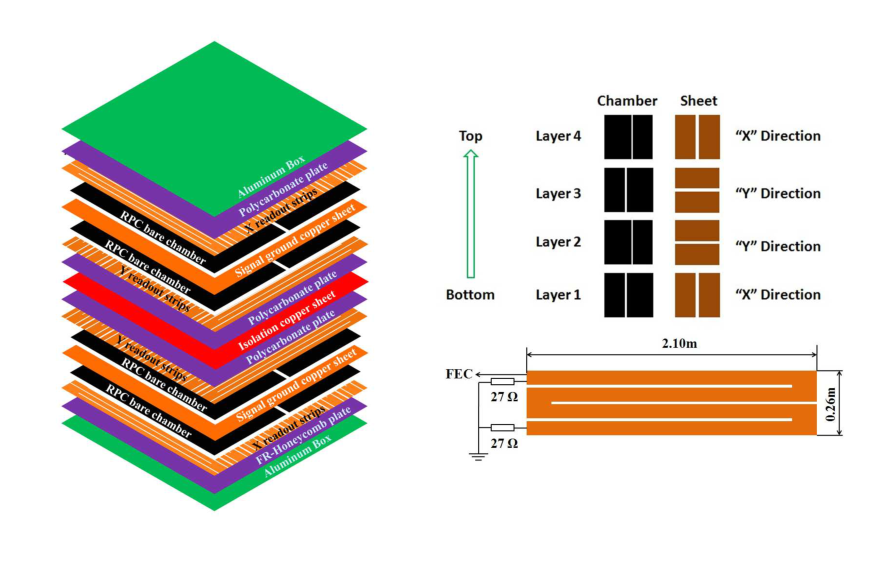
\includegraphics[width=0.9\textwidth]{figures/chap5/RPC_inner_structure.eps}
	\caption{Left: the inner structure of a RPC module. Right: the arrangement of RPC bare chambers for each layer and the zigzag structure of a readout strip.}
	\label{fig:module_inner_structure}
\end{figure}
A RPC module is composed of 4 layers of RPC bare chambers. Each layer is formed by 2 RPC bare chambers with the same length but different width. The larger RPC bare chamber has a dimension of 2.1 m $\times$ 1.1 m. The smaller one has a dimension of 2.1 m $\times$ 1.0 m. From bottom to top, the sizes of the RPC bare chambers alternates so as to offset the dead region due to the edges of the bare chambers. Each RPC layer is equipped with a 2.1 m $\times$ 2.1 m copper-clad FR-4 readout plane consisting of 8 readout strips resulting in a strip dimension of 26 cm $\times$ 210 cm. The strips are of a zigzag design which is equivalent to a strip 6.5 cm wide and 8.4 m long (see bottom right of Figure~\ref{fig:module_inner_structure}). The zigzag design in effect changes the impedance so as to give a larger and narrower pulse because of the change in the impedance of the transmission line~\cite{Riegler2002}. One end of the strip is connected to the RPC Front End Card (FEC, see Section~\ref{sec:RPC_electronics}) while the other end is connected to a ground by two 27 $\Omega$ resistors, a value determined in bench tests (see Figure~\ref{fig:RPC_signal}(a)). Figure~\ref{fig:RPC_signal}(b) shows some signals read out by the oscilloscope in bench tests. The signal threshold in Daya Bay's physics data taking is set at 30 mV.
\begin{figure}
  \centering
  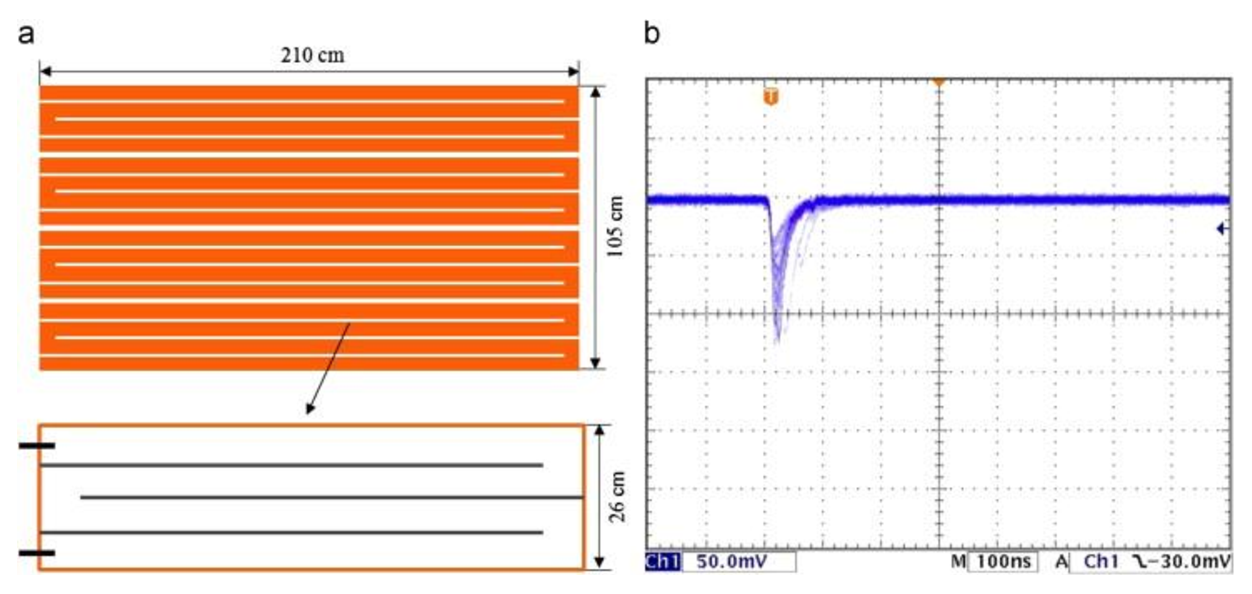
\includegraphics[width=0.8\textwidth]{figures/chap5/RPC_signal.eps}
  \caption{(a) Readout zigzag structure and the signal termination. (b) Readout signals on the oscilloscope.}
  \label{fig:RPC_signal}
\end{figure}
The 4 readout layers are oriented, from bottom to top, in the $x$, $y$, $y$, $x$ directions as shown in Figure~\ref{fig:module_inner_structure}. With this readout arrangement, the position of the incident muon can be determined by identifying the intersection of the $x$ and $y$ strips.


\section{Gas and High Voltage System}
The RPCs operate in streamer mode with a gas mixture of Ar:C$_2$H$_2$F$_4$:i-C$_4$H$_{10}$:SF$_6$=65.5:30:4:0.5. Each site has a gas system which consists of gas cylinders, gas mixing and distribution systems, fire safety monitoring systems, and gas chromatography (GC) systems. The flow rate of each site is about 1 RPC volume exchange per day, and is controlled by an electronic mass flow control system.

The high voltage (HV) system includes a CAEN HV mainframe for supplying the operating 7600 V HV, the fanout boxes for HV channel multiplication, and the HV interface boxes for connecting the HV to the RPC module. The HV channels from the mainframe are controlled and monitored remotely by the Daya Bay Detector Control System (DCS). There is also an interlock functionality to ensure safe operation: if there are alarm signals from the gas system, the HV DCS sends out warnings to the monitors in the control room, and allows 30 minutes for troubleshooting before the HV gets automatically shut down.


\section{RPC Readout Electronics}\label{sec:RPC_electronics}
Figure~\ref{fig:RPC_electronics} shows the architecture of the RPC readout electronics. The readout system consists of four boards and modules, namely the Front-End Card (FEC), the ReadOut Transceiver (ROT), the ReadOutModule (ROM), and the RpcTroggerModule (RTM). The number of each kind of board or module installed in each hall is summarized in Table~\ref{table:num_installed}.
\begin{figure}
	\centering
	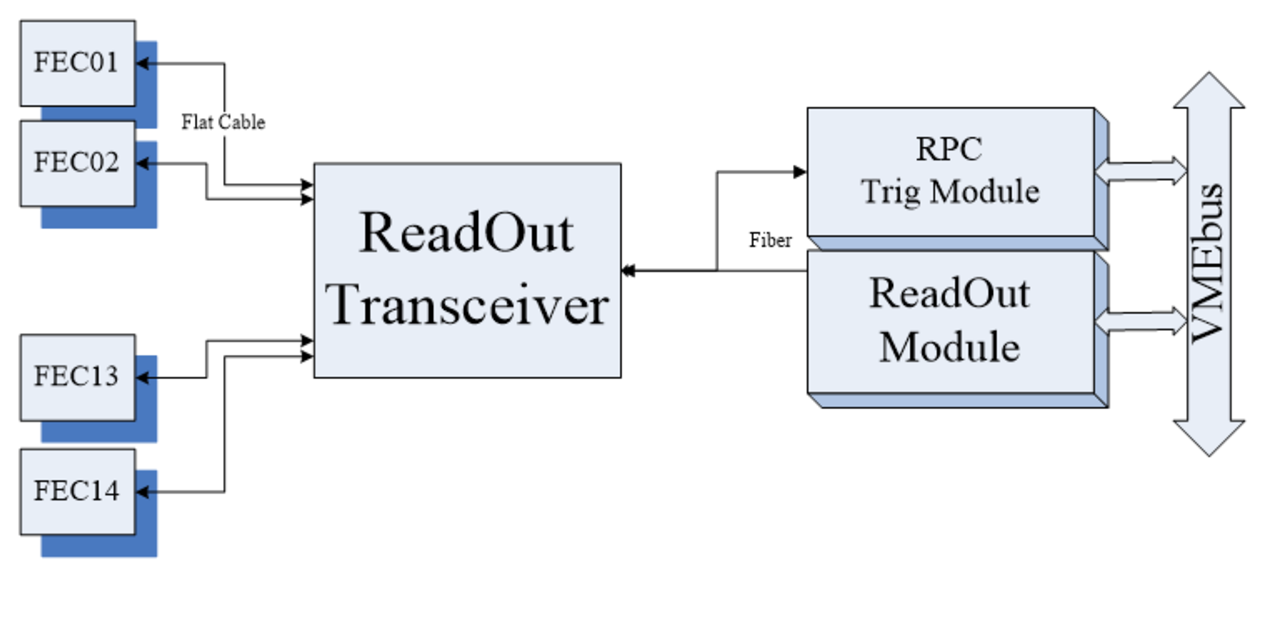
\includegraphics[width=.75\textwidth]{figures/chap5/RPC_Readout.eps}
	\caption{Architecture of the RPC readout electronics.}
	\label{fig:RPC_electronics}
\end{figure}
\begin{table}
	\centering
	\begin{tabular}{ccc}
		\hline
		board or module & near hall & far hall \\
		\hline
		FEC & 54 & 81 \\
		ROT & 4 & 6 \\
		ROM & 1 & 1 \\
		RTM & 1 & 1 \\
		\hline
	\end{tabular}
	\caption{Number of boards/modules installed in each hall.}
	\label{table:num_installed}
\end{table}
Daya Bay's FEC is the signal front end readout card for RPC detectors. Each card collects signals from the 32 channels of a RPC module. The FEC amplifies the signal, and generates a digital signal for signals above 30 mV threshold, and adds timestamp from the system clock. FECs generate local triggers with different modes specified by input signals and pass them to ROT. Signal transmission from FEC to ROT is done with flat cables. There are two kinds of local trigger modes, 2/4 and 3/4. In 2/4 mode, triggers are issued if at least two layers of RPCs are fired. In 3/4 mode, triggers are issued if at least three layers of RPCs are fired. In Daya Bay's physics data taking, since the amount of data generated by 2/4 mode takes too much storage and is mostly due to non-physics events, 3/4 trigger mode is used.
The ROT transmits readout data and configuration data between FEC and ROM. In addition, ROT transmits local trigger signals to RTM. Each ROT accepts up to 15 FEC signals, packs up data from 15 cards, and passes them to ROM and RTM through optical links. The ROM and RTM then process the data and issue triggers.


\section{Event Reconstruction}
In this study the yield of muon-induced neutrons is measured by constructing fiducial volumes around the muon tracks. Only neutrons captured inside the fiducial volume are counted. In this section the event vertices and the muon tracks are discussed.

\subsection{AD Event Reconstruction}
In this study, the energy and vertex of an AD event are obtained by the ``AdSimple'' reconstruction algorithm~\cite{docdb7334}. AdSimple reconstructs the energy and vertex of a point-like event such as the neutron capture on Gd.
\paragraph{Vertex Reconstruction} The vertex reconstruction in AdSimple involves two steps. First the charge-weighted mean from all PMTs is used to obtain the preliminary value. Then a correction scheme obtained from MC simulation is applied to the preliminary value.
The preliminary vertex is obtained by
\begin{equation}
	\vec{r}_{coc}=\frac{\sum\limits_iQ_i\vec{r}_i}{\sum\limits_iQ_i}
\end{equation}
where $\vec{r}_{coc}$ is the center of charge position, $i$ runs over all 192 8" PMTs, $Q_i$ is the charge received by the $i$th PMT, and $\vec{r}_i$ is the position of the PMT.
As a result of reflectors on the top and bottom of the AD, it is found that the the center of charge positions $\vec{r}_{coc}$ are pulled to the center of the AD. This bias can be corrected by the IBD Monte Carlo simulation including both positron and neutron events. The OAV is divided into bins in both the radial $\rho$ and the vertical $z$ directions. Then quantities $\Delta \rho$ and $\Delta z$ are defined\footnote{\begin{eqnarray}
\Delta \rho &=& \vec{\rho}_{true}\cdot \frac{\vec{\rho}_{coc}}{\rho_{coc}}-\rho_{coc} \\
\Delta z &=& z_{true}-z_{coc}
\end{eqnarray}} representing the deviation of $\vec{r}_{coc}$ from the true position $\vec{r}_{true}$. For each bin the average values of $\Delta \rho$ and $\Delta z$ are calculated, and these values are assigned to the center of the bin. To obtain $(\Delta\rho,\Delta z)$ for all $(\rho,z)$, an interpolation is applied. Finally the correction is added to each $\vec{r}_{coc}$ to obtain the reconstructed vertex $\vec{r}_{rec}$. The position resolution of this algorithm for Gd captured neutrons is $\sim$20 cm in both $\rho$ and $z$ directions.

\paragraph{Energy Reconstruction} The AdSimple energy reconstruction involves three steps. The first step is the determination of the total charge deposited in the detector recorded by PMTs. The second step is the conversion of this charge to a physical energy scale. \mbox{Finally}, a correction is applied to account for the detector non-uniformity.
Concerning the total charge determination, for an AD trigger the energies deposited in all PMTs are all counted. For each PMT, the pedestal subtracted ADC value is converted into number of photoelectrons (pe's) using the calibration constants specific to individual channels in the offline database which is updated weekly. Only PMT hits in the time window $[-1650ns,-1250ns]$ with respect to the time the trigger is issued are summed to obtain the PMT charge for each PMT.
%The reason is that if all PMT hits in a readout are used, it will give a worse energy resolution due to the inclusion of too many dark hits or afterpulses.

Once the total charge sum is obtained for an AD trigger in the units of photoelectrons, the charge has to be converted into real physical energy scale. Here the spallation neutrons are used to set the photoelectron to energy scale. The spallation neutrons captured on Gd is uniformly distributed in the GdLS, providing access to the whole detector active volume. The 8 MeV peak is close to the lower bound of the delayed signal energy cut which constitute a dominant systematic uncertainty. The number of photoelectrons divided by 8 MeV then serves as the energy scale constant for the AD. For all ADs, this value is about 170 photoelectrons/MeV. Finally the energy scale as a function of $r$ and $z$ are studied and corrected.

In this study, muon-induced neutrons are selected by an energy cut with energies reconstructed by AdSimple algorithm. Also, the capture sites of neutrons are required to be within a fiducial volume with capture vertices reconstructed by this algorithm as well.

\subsection{Muon Track Reconstruction}
In this study, muon tracks are reconstructed by the muon system. The muon system consists of three independent detectors, the RPC, the IWS, and the OWS. The RPC by design can reconstruct the muon incident position simply by identifying the intersection of the fired strips which gives a point in the muon track. On the other hand, the two PMT-based Cherenkov detectors can each offer an reconstructed point in the muon track by the PMT charge pattern. Thus, from the muon system alone, at most four points can be obtained if the muon passes through the telescope RPC, the RPC array, the IWS, and the OWS. A muon track can be reconstructed utilizing those points reconstructed with the individual muon subsystems.

\subsubsection{RPC Vertex Reconstruction}
RPC readout strips by design are used for muon point reconstruction. Since in the physics data taking the 3/4 trigger scheme is used, there is at least a pair of $x$ and $y$ strips from adjacent layers, cf. Figure~\ref{fig:module_inner_structure}. The eight $x$ strips and the eight $y$ strips divide the surface of a RPC module into 64 ``patches''. One can then assign the coordinate of the center of the patch formed by the fired strips as the reconstructed point. Figure~\ref{fig:RPC_event} is an example of a real RPC event. If in the same readout layer several contiguous strips, which we call clusters, are fired, the centroid of them is used. If two layers with the same strip orientation, say the $x$ layers, contain fired strips, the centroid of the layer centroids is used as the reconstructed coordinate.
\begin{figure}
	\centering
	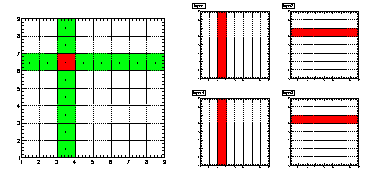
\includegraphics[width=0.9\textwidth]{figures/chap5/RPC_event.pdf}
	\caption{A RPC event. Left: multiplicity of fired patches. Right: fired strips in each layer.}
	\label{fig:RPC_event}
\end{figure}

Some rarer situations have to be considered here. If in the same layer several disjoint clusters exist, ``ghost hits'' are formed, i.e., there are multiple intersection points of $x$ and $y$ clusters. For Daya Bay, it is difficult to discriminate ghost hits from real hits. Fortunately the fraction of events with ghost hits is very small. There are also crosstalk events due to strong signals penetrating the copper ground plane in the center of the module. For such kind of events, most strips ($>4$) in the central two $y$ layers have hits. To remove the crosstalk events, a simple cluster size cut with at most two contiguous strips removes them effectively. Based on one day of data, the approximate distributions of the RPC hit pattern are
\begin{itemize}
	\item 97\% of the clusters are of size 1 strip,
	\item 96\% of the triggers contain only 1 muon per module,
	\item 97\% of the triggers contain only 1 module in the entire hall,
	\item 99\% of the events fire vertical clusters.
\end{itemize}
From these distributions we see that the RPC muon detector in fact serves as a high efficiency ($>95\%$~\cite{Ning2013}), low noise muon tracking detector.

\subsubsection{Water Shield Vertex Reconstruction}
The algorithm for water pool vertex reconstruction is dubbed ``PoolSimple''~\cite{docdb7838}. The water shields detect relativistic charged particles through the emission of Cherenkov radiation when the speed of the charged particle is larger than the speed of light in water. Unlike the uniform emission of scintillation light produced by the AD events, the Cherenkov photons are emitted in a cone relative to the direction of the charged particle. For water, this angle is about 41\textdegree. A complete water Cherenkov reconstruction algorithm should employ the timing information of PMT hits. However, getting the timing calibration done correctly is a rather involved task and the current preliminary results~\cite{docdb7696} still have room to improve. This algorithm uses only the PMT charge and hit pattern to reconstruct the muon track, and it turns out to have a reasonably good resolution.

As in the AD vertex reconstruction, a charge-weighted mean is used as the reconstructed vertex,
\begin{equation}
	\vec{r}_{rec}=\frac{\sum\limits_{i=1}^{n_{max}}Q_i\vec{r}_i}{\sum\limits_{i=1}^{n_{max}}Q_i}
\end{equation}
where $Q_i$ is the charge the $i$th PMT receives, and $\vec{r}_i$ is the position vector of that PMT. $n_{max}$ is the first $n_{max}$ PMTs with the largest received charge, and is determined by simulation. The idea is that the closer the PMT is to the muon track the more light it will receive. Also since the Cherenkov radiation is directional, the PMTs in proximity to the PMT with largest charge receive more light than PMTs far from the muon track. Therefore only selecting a number of PMTs with the largest charge provides better resolution than taking all PMTs in the pool. Since each water pool is regarded as an independent detector, this algorithm gives two reconstructed vertices, one for each pool.

The resolution of this algorithm is obtained by simulation. One can determine the distance from the center of the OWS to the true track. Call this parameter $d_{true}$. The same point to the reconstructed track is $d_{rec}$. One can plot the distribution of $d_{rec}-d_{true}$. The position resolution obtained from the distribution is $\sim$60 cm shown in Figure~\ref{fig:WS_resolution}.
\begin{figure}
	\centering
	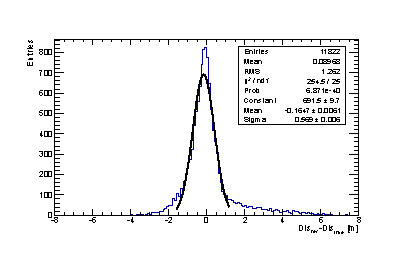
\includegraphics[width=0.7\textwidth]{figures/chap5/WS_resolution.eps}
	\caption{The distribution of $d_{rec}-d_{true}$.}
	\label{fig:WS_resolution}
\end{figure}

\subsubsection{Muon Track Reconstruction}
When a muon passes through the Daya Bay muon system, depending on the geometry of the track and the muon detectors, at most four points can be reconstructed if the telescope RPC is also hit by the muon. Since RPCs have a superior resolution than the water pool, in this study only muons having an RPC trigger and a water pool vertex are considered. Furthermore, since ADs are sitting in the inner water pool, the PMTs on the bottom of the pool are shadowed by the ADs. This situation known as the AD shadowing effect. The result is that the bottom PMTs don't see enough light, pulling the reconstructed vertex towards the wall of the water pool. Contrarily, the outer water pool doesn't suffer from this effect. Consequently, the muon track used in this study is obtained by connecting the RPC and the OWS vertices.